% This file was created by matlab2tikz.
%
%The latest updates can be retrieved from
%  http://www.mathworks.com/matlabcentral/fileexchange/22022-matlab2tikz-matlab2tikz
%where you can also make suggestions and rate matlab2tikz.
%
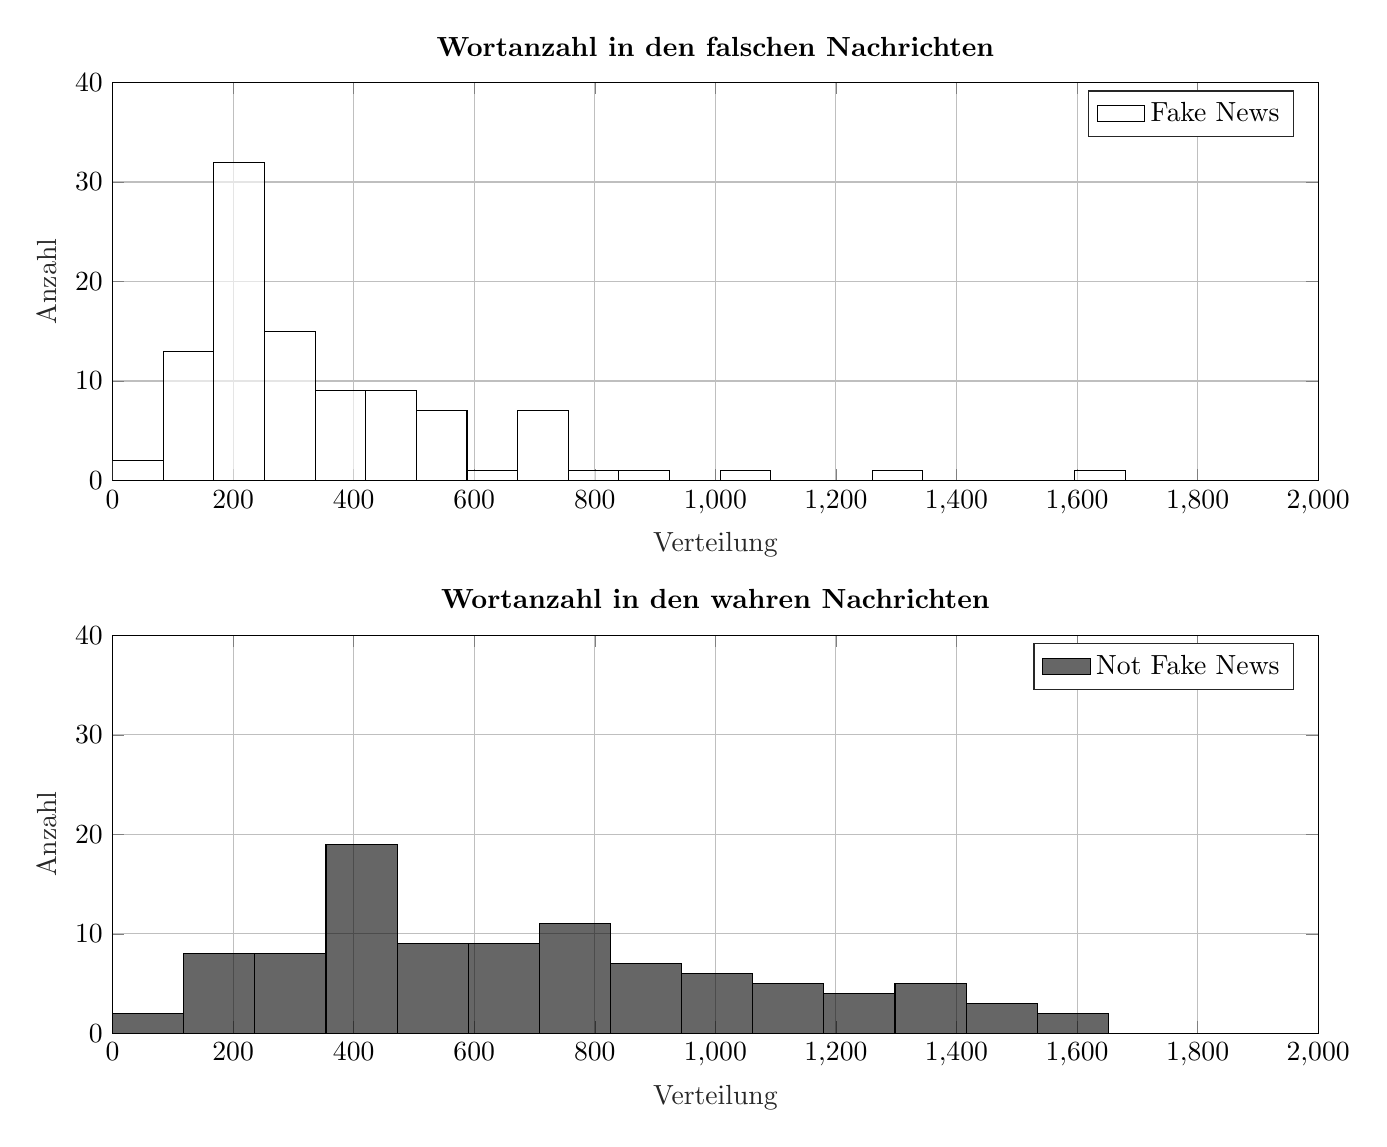
\begin{tikzpicture}

\begin{axis}[%
width=6.028in,
height=1.99in,
at={(1.011in,3.406in)},
scale only axis,
xmin=0,
xmax=2000,
xlabel style={font=\color{white!15!black}},
xlabel={Verteilung},
ymin=0,
ymax=40,
ylabel style={font=\color{white!15!black}},
ylabel={Anzahl},
axis background/.style={fill=white},
title style={font=\bfseries},
title={Wortanzahl in den falschen Nachrichten},
xmajorgrids,
ymajorgrids,
legend style={legend cell align=left, align=left, draw=white!15!black}
]
\addplot[ybar interval, fill=white, fill opacity=0.6, draw=black, area legend] table[row sep=crcr] {%
x	y\\
0	2\\
84	13\\
168	32\\
252	15\\
336	9\\
420	9\\
504	7\\
588	1\\
672	7\\
756	1\\
840	1\\
924	0\\
1008	1\\
1092	0\\
1176	0\\
1260	1\\
1344	0\\
1428	0\\
1512	0\\
1596	1\\
1680	1\\
};
\addlegendentry{Fake News}

\end{axis}

\begin{axis}[%
width=6.028in,
height=1.99in,
at={(1.011in,0.642in)},
scale only axis,
xmin=0,
xmax=2000,
xlabel style={font=\color{white!15!black}},
xlabel={Verteilung},
ymin=0,
ymax=40,
ylabel style={font=\color{white!15!black}},
ylabel={Anzahl},
axis background/.style={fill=white},
title style={font=\bfseries},
title={Wortanzahl in den wahren Nachrichten},
xmajorgrids,
ymajorgrids,
legend style={legend cell align=left, align=left, draw=white!15!black}
]
\addplot[ybar interval, fill=black, fill opacity=0.6, draw=black, area legend] table[row sep=crcr] {%
x	y\\
0	2\\
118	8\\
236	8\\
354	19\\
472	9\\
590	9\\
708	11\\
826	7\\
944	6\\
1062	5\\
1180	4\\
1298	5\\
1416	3\\
1534	2\\
1652	0\\
1770	0\\
1888	0\\
2006	0\\
2124	1\\
2242	1\\
2360	1\\
};
\addlegendentry{Not Fake News}

\end{axis}
\end{tikzpicture}%